\chapter{E-Puck}
\label{chap:epuck}
  An object of interest of a this thesis is a programming of the e-Puck robot.
  In this chapter the~robot and its design is introduced. 
  Then in Section \ref{sec:mechanical} the chapter continues 
  with~description e-Puck's mechanical design. Section \ref{sec:sensors} is devoted to e-Puck's sensors and actuators. 

  We focus on a programmer's point of view of e-Puck qualities.
  For each sensor its functions, acceptable values and typical use is shortly presented. 
  The chapter finishes with a description of a e-Puck's camera and outlining other e-Puck abilities.
\section{Origin of e-Puck}
\label{sec:mechanical}
  Motivation for a new robot arose from an absence of a very small educational robot,
  which is can be used for education in many research areas.
  E-Puck was developed in summer of 2004 at the �cole Polytechnique F�d�rale de Lausanne (EPFL) 
  as an open tool. E-Puck designers used open software and hardware development model. 
  E-Puck can be applied in automatic control, signal processing or 
  distributed intelligent system research. E-Puck's structure is robust and simple to care about, 
  because e-Puck is intended to be used by students.
  Designers of e-Puck tried to use manufacturing components as much as possible 
  in order to keep the price low.		 
  
  Since 2006 the first generation of e-Pucks was replaced by the second generation.
  So far, more than 2000 e-Pucks in version 2 have been manufactured.
  There are several distributors for Switzerland and America, one is in Japan
  \footnote{\url{http://www.roadnarrows.com/robotics/}, \url{http://www.aai.jp/}, \url{http://www.k-team.com/},
  \url{http://www.cyberbotics.com/products/robots/e-puck.html}, \url{http://www.gctronic.com/},
  \url{http://www.aai.ca/robots/e-puck.html}}.
  The price of e-Puck should be between 450 and 550 Eurors. 
  %\textgreek{\euro}.%todo znak eura
  %\usepackage[greek,<optional other language>]{babel} for euro symbol

\section{Mechanical Design}
\label{sec:mechanical}
  %\input{epuck_str.TpX} %pouzite \cite{robotica2009}
  \begin{figure}[!hbp]
  \centering
  \ifpdf
    \setlength{\unitlength}{1bp}%
    \begin{picture}(232.44, 320.96)(0,0)
    \put(0,0){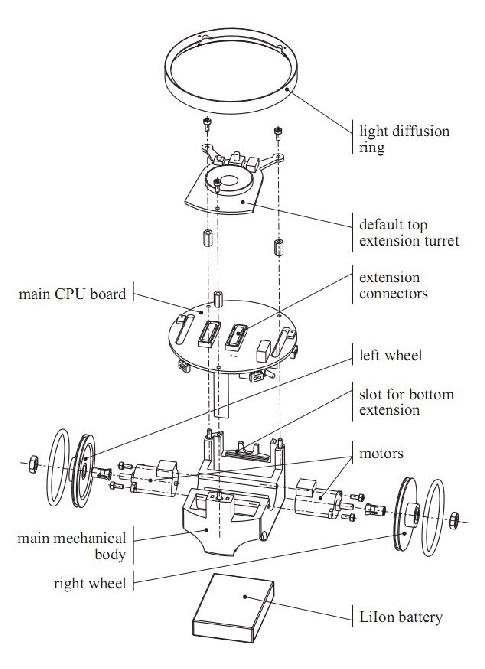
\includegraphics{epuck_str.pdf}}
    \end{picture}%
  \else
    \setlength{\unitlength}{1bp}%
    \begin{picture}(232.44, 320.96)(0,0)
    \put(0,0){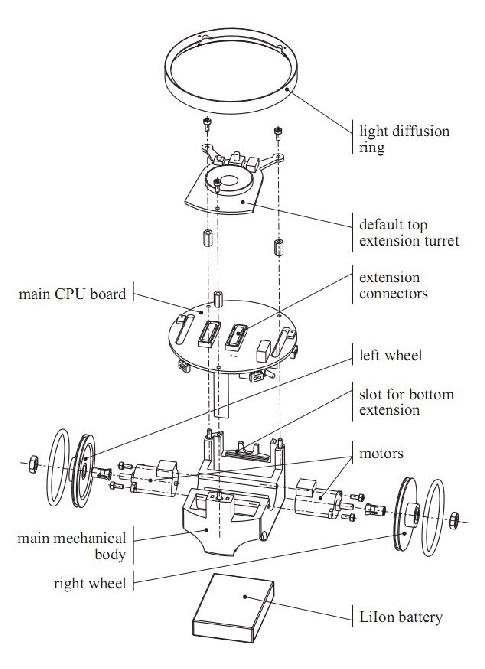
\includegraphics{epuck_str}}
    \end{picture}%
  \fi
  \caption{\label{pic:epuck_str}%
   Epuck structure \cite{robotica2009}}
  \end{figure}

  The mechanical design of e-Puck is shown in Figure~\ref{pic:epuck_str}.
  It consists of a rounded transparent body, a battery, two stepper motors, 
  wheels , a printed circuit board, plastic ring of LEDs, 
  a camera and a default extension board.
  There are extensions like floor sensors, a rotating scanner or a turret with linear cameras,
  which can scale up e-Puck's sensors. If we are talking about e-Puck in this thesis,
  it is meant e-Puck with the default extension only.
  
  A default robot is more than 60 mm 
  high and it has a diameter of 75 mm. 
  The battery is placed in the bottom and can be easily extracted and recharged separately.
  Two stepper motors with wheels are screwed to a plastic body and are located on axis of e-Puck
  in order to allow robot turn around on place. Wheels have the diameter of 41 mm and the perch is 53 mm.
  Printed circuit board is fixed to the top of the body and a ring of LEDs' is mounted around the board.
  A camera is placed on the front side of robot lying on the axis between the wheels.
  The extension board covers the main printed circuit board.
\section{Sensors, actuators and heart of the robot}
\label{sec:sensors}
  Sensors and actuators determine the possible robot usage.
  Luckily, e-Puck has a lot of sensors of different kinds and is equipped with typical actuators.
  The following paragraphs shortly describe e-Puck's sensors and actuators and mention a few problems 
  with transmitting data between the robot and PC using {\it BTCom}. {\it BTCom} protocol is used by {\it Elib} library,
  so {\it Elib} is to some extent dependent on {\it BTCom}.
  The actuators consist of motors, 8 red LEDs on perimeter, 4 green body LEDs,
   which are turned on/off together, a front LED and a speaker.
   
  Stepper motors are a great advantage of e-Puck, because the motion of wheel can be split
  into small steps. One wheel revolution corresponds to 1000 steps of motor. The 
  diameter of the wheel is 41 mm. If the wheel makes one revolution, the wheel goes 128.8 mm. 
  In conclusion a thousand of steps matches 128.8 mm of linear movement and one step is 0.1288 mm. 
  Motors are equipped with encoders and the motors are very accurate, 
  which in combination with simple odometry really helps in localization tasks.
  A nice feature of encoders is that their value can be set at any time.
  The maximum speed of the motors is one revolution per second in both directions.
  {\it BTCom} allows a programmer to set the speed of motors and also get and set the values
  of encoders.
   
  All e-Puck LEDs can be used for debugging or for making robot visible to other devices.
  Furthermore, the front LED is usually used to illuminate the terrain in front of  e-Puck.
  Each LED can be turned off, turned on or set to an inverse state.
  
  Three axis accelerometers are placed inside the robots body. In the rest position
  the accelerometers measure the slant of e-Puck. They can also measure acceleration of e-Puck
  and for example detect a collision or a falling state of e-Puck. 
%	There is no problem with using accelerometer via {\it BTCom}.
  
  Infra Red (IR) sensors are typical sensors for mobile robotics. E-Puck has eight of them.
  Four are located in the front part of e-Puck, two are on both sides, two on back side.
  Sensors work in two modes. First they measure ambient infra red light.
  In the second mode IR sensors emit IR light and they measure reflected light, so 
  they can detect close obstacles.
  Both functions are available in {\it BTCom}. 				
  Calibration of sensors increases the precision of detecting near obstacles.
  Infra red sensors are capable of recognising an obstacle at a distance 4 cm.
  
  The speaker together with microphones are suitable communication tools between
  the people and e-Puck.
  On the other hand, a limited processing power of e-Puck does not allow to store and
   play complicated sounds. It is also impossible to use a speaker with microphones to speech
   recognition due to insufficient processing power.
  Despite the limitation of processing power the microphones can be easily used to locate
  the source of sound via amplitude measurement, because the microphones are placed near the perimeter
  in a triangle. Microphones measure current amplitude of sound. As exact distances between microphones 
  are known, we can compute frequency of the sound using Fast Fourier Transformation (FFT).
  Digital Signal Processor (DSP) is suitable for computing FFT,
   which will be introduced below in this chapter.
  Maximal acquisition speed is 33 kHz. 
  For more information see \cite{sound}.
  
  \begin{remark}
  A program which uses {\it BTCom} can capture values of amplitude only in irregular intervals, so 
  it is not possible to compute frequency of sound by running FFT on Personal Computer. 
%  However to locate the source of sound is still possible.
  \end{remark}
  
  %\chapter{E-Puck}
\label{chap:epuck}
  An object of interest of a this thesis is a programming of the e-Puck robot and e-Puck itself.
  In this chapter e-Puck robot and its design is introduced. 
  Then in Section \ref{sec:sensors} the chapter continues 
  with~description e-Puck's mechanical design and stepper motors in Section
  \ref{sec:mechanical}. 
  We focus on a programmer's point of view of e-Puck qualities.
  For each sensor its functions, acceptable values and typical use is shortly presented. 
  The chapter finishes with a description of a e-Puck's camera and outlining other e-Puck abilities.
\section{Origin of e-Puck}
\label{sec:mechanical}
  Motivation for a new robot arose from an absence of a very small educational robot,
  which is sufficiently efficient, and can be used for education in many research areas.
  E-Puck was developed in summer of 2004 at the �cole Polytechnique F�d�rale de Lausanne (EPFL) 
  as an open tool. E-Puck designers used open software and hardware development model. 
  E-Puck can be applied in automatic control, signal processing or 
  distributed intelligent system research. E-Puck's structure is robust and simple to care about, 
  because e-Puck is intended to be used by students.
  Designers of e-Puck tried to use manufacturing components as much as possible 
  in order to keep the price low.		 
  
  Since 2006 the first generation of e-Pucks was replaced by the second stable generation.
  So far, more than 2000 robots have been manufactured.
  There are several distributors for Switzerland and America, one is in Japan
  \footnote{\url{http://www.roadnarrows.com/robotics/}, \url{http://www.aai.jp/}, \url{http://www.k-team.com/},
  \url{http://www.cyberbotics.com/products/robots/e-puck.html}, \url{http://www.gctronic.com/},
  \url{http://www.aai.ca/robots/e-puck.html}}.
  The price of e-Puck should be between 450 and 550 Eurors. 
  %\textgreek{\euro}.%todo znak eura
  %\usepackage[greek,<optional other language>]{babel} for euro symbol

\section{Mechanical Design}
\label{sec:mechanical}
  %\input{epuck_str.TpX} %pouzite \cite{robotica2009}
  \begin{figure}[!hbp]
  \centering
  \ifpdf
    \setlength{\unitlength}{1bp}%
    \begin{picture}(232.44, 320.96)(0,0)
    \put(0,0){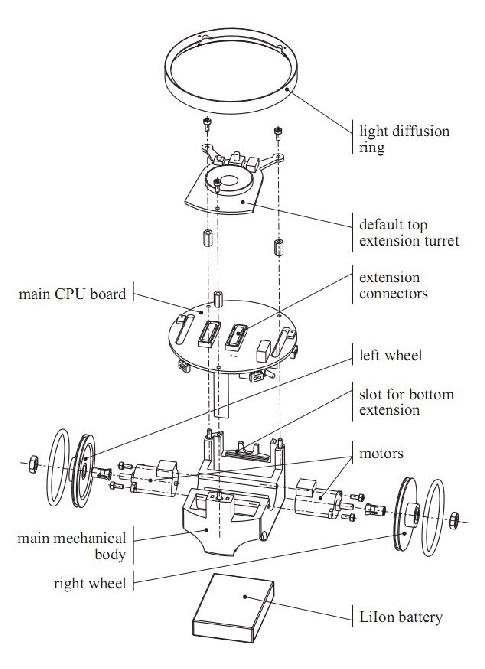
\includegraphics{epuck_str.pdf}}
    \end{picture}%
  \else
    \setlength{\unitlength}{1bp}%
    \begin{picture}(232.44, 320.96)(0,0)
    \put(0,0){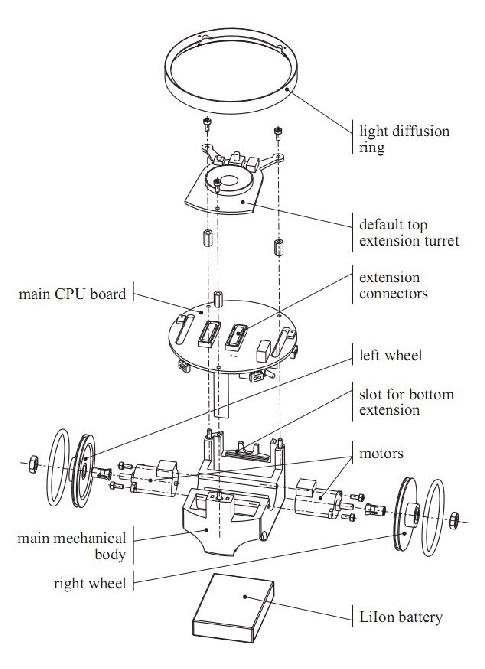
\includegraphics{epuck_str}}
    \end{picture}%
  \fi
  \caption{\label{pic:epuck_str}%
   Epuck structure \cite{robotica2009}}
  \end{figure}

  The mechanical design of e-Puck is shown in Figure ~\ref{pic:epuck_str}.
  It consists of a rounded transparent body, a battery, two stepper motors with
  wheels on their axis, a printed circuit board, plastic ring of LEDs, 
  a camera and a default extension board.
  There are extensions like floor sensors, a rotating scanner or a turret with linear cameras,
  which can scale up e-Puck's sensors. If we are talking about e-Puck in this thesis,
  it is meant e-Puck with the default extension only.
  
  A default robot is more than 60 mm 
  high and it has a diameter of 75 mm. 
  The battery is placed in the bottom and can be easily extracted and recharged separately.
  Two stepper motors with wheels are screwed to a plastic body and are located on axis of e-Puck
  in order to allow robot turn around on place. Wheels have the diameter of 41 mm and the perch is 53 mm.
  Printed circuit board is fixed to the top of the body and a ring of LEDs' is mounted around the board.
  A camera is placed on the front side of robot lying on the axis between the wheels.
  The extension board covers the main printed circuit board.
\section{Sensors, actuators and heart of the robot}
\label{sec:sencors}
  Sensors and actuators determine the possible robot usage.
  Luckily, e-Puck has a lot of sensors of different kinds and is equipped with typical actuators.
  The following paragraphs shortly describe e-Puck's sensors and actuators and mention a few problems 
  with transmitting data between the robot and PC using {\it BTCom}. {\it BTCom} protocol is used by {\it Elib},
  so {\it Elib} is to some extent dependent on {\it BTCom}.
  The actuators consist of motors, 8 red LEDs on perimeter, 4 green body LEDs,
   which are turned on/off together, a front LED and a speaker.
   
  Stepper motors are a great advantage of e-Puck, because the motion of wheel can be split
  into small steps. One wheel revolution corresponds to 1000 steps of motor. The 
  diameter of the wheel is 41 mm. If the wheel makes one revolution, the wheel goes 128.8 mm. 
  In conclusion a thousand of steps matches 128.8 mm of linear movement and one step is 0.1288 mm. 
  Motors are equipped with encoders and the motors are very accurate, 
  which in combination with simple odometry really helps in localization tasks.
  A nice feature of encoders is that their value can be set at any time.
  The maximum speed of the motors is one revolution per second in both directions.
  {\it BTCom} allows a programmer to set the speed of motors and also get and set the values
  of encoders.
   
  All e-Puck LEDs can be used for debugging or for making robot visible to other devices.
  Furthermore, the front LED is usually used to illuminate the terrain in front of  e-Puck.
  Each LED can be turned off, turned on or set to an inverse state.
  
  Three axis accelerometers are placed inside the robots body. In the rest position
  the accelerometers measure the slant of e-Puck. They can also measure acceleration of e-Puck
  and for example detect a collision or a falling state of e-Puck. 
%	There is no problem with using accelerometer via {\it BTCom}.
  
  Infra Red (IR) sensors are typical sensors for mobile robotics. E-Puck has eight of them.
  Four are located in the front part of e-Puck, two are on both sides, two on back side.
  Sensors work in two modes. First they measure ambient infra red light.
  In the second mode IR sensors emit IR light and they measure reflected light, so 
  they can detect close obstacles.
  Both functions are available in {\it BTCom}. 				
  Calibration of sensors increases the precision of detecting near obstacles.
  Infra red sensors are capable of recognising an obstacle at a distance 4 cm.
  
  The speaker together with microphones are suitable communication tools between
  the people and e-Puck.
  On the other hand, a limited processing power of e-Puck does not allow to store and
   play complicated sounds. It is also impossible to use a speaker with microphones to speech
   recognition due to insufficient processing power.
  Despite the limitation of processing power the microphones can be easily used to locate
  the source of sound via amplitude measurement, because the microphones are placed near the perimeter
  in a triangle. Microphones measure current amplitude of sound. As exact distances between microphones 
  are known, we can compute frequency of the sound using Fast Fourier Transformation (FFT).
  Digital Signal Processor (DSP) is suitable for computing FFT,
   which will be introduced below in this chapter.
  Maximal acquisition speed is 33 kHz. 
  For more information see \cite{sound}.
  
  A program which uses {\it BTCom} can capture values of amplitude only in irregular intervals, so 
  it is not possible to compute frequency of sound by running FFT on Personal Computer. 
  However to locate the source of sound is still possible.
  
  %\chapter{E-Puck}
\label{chap:epuck}
  An object of interest of a this thesis is a programming of the e-Puck robot and e-Puck itself.
  In this chapter e-Puck robot and its design is introduced. 
  Then in Section \ref{sec:sensors} the chapter continues 
  with~description e-Puck's mechanical design and stepper motors in Section
  \ref{sec:mechanical}. 
  We focus on a programmer's point of view of e-Puck qualities.
  For each sensor its functions, acceptable values and typical use is shortly presented. 
  The chapter finishes with a description of a e-Puck's camera and outlining other e-Puck abilities.
\section{Origin of e-Puck}
\label{sec:mechanical}
  Motivation for a new robot arose from an absence of a very small educational robot,
  which is sufficiently efficient, and can be used for education in many research areas.
  E-Puck was developed in summer of 2004 at the �cole Polytechnique F�d�rale de Lausanne (EPFL) 
  as an open tool. E-Puck designers used open software and hardware development model. 
  E-Puck can be applied in automatic control, signal processing or 
  distributed intelligent system research. E-Puck's structure is robust and simple to care about, 
  because e-Puck is intended to be used by students.
  Designers of e-Puck tried to use manufacturing components as much as possible 
  in order to keep the price low.		 
  
  Since 2006 the first generation of e-Pucks was replaced by the second stable generation.
  So far, more than 2000 robots have been manufactured.
  There are several distributors for Switzerland and America, one is in Japan
  \footnote{\url{http://www.roadnarrows.com/robotics/}, \url{http://www.aai.jp/}, \url{http://www.k-team.com/},
  \url{http://www.cyberbotics.com/products/robots/e-puck.html}, \url{http://www.gctronic.com/},
  \url{http://www.aai.ca/robots/e-puck.html}}.
  The price of e-Puck should be between 450 and 550 Eurors. 
  %\textgreek{\euro}.%todo znak eura
  %\usepackage[greek,<optional other language>]{babel} for euro symbol

\section{Mechanical Design}
\label{sec:mechanical}
  %\input{epuck_str.TpX} %pouzite \cite{robotica2009}
  \begin{figure}[!hbp]
  \centering
  \ifpdf
    \setlength{\unitlength}{1bp}%
    \begin{picture}(232.44, 320.96)(0,0)
    \put(0,0){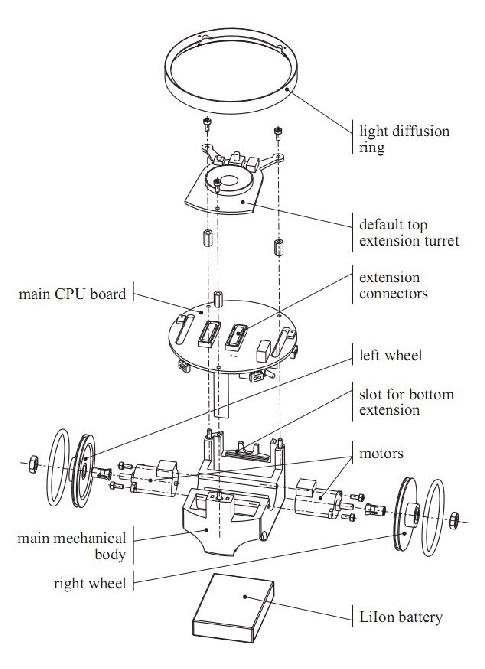
\includegraphics{epuck_str.pdf}}
    \end{picture}%
  \else
    \setlength{\unitlength}{1bp}%
    \begin{picture}(232.44, 320.96)(0,0)
    \put(0,0){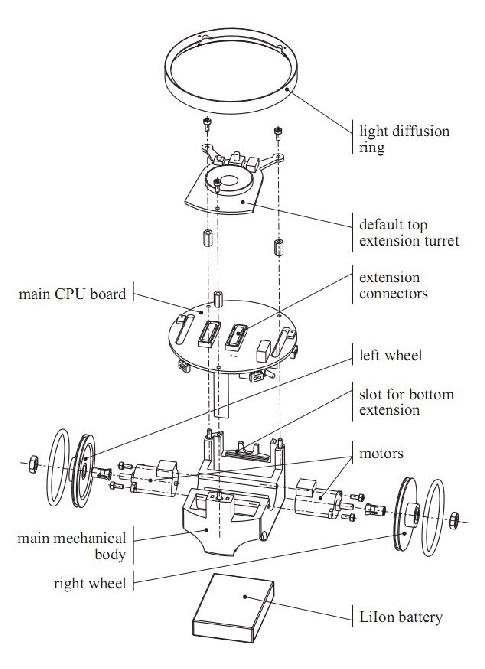
\includegraphics{epuck_str}}
    \end{picture}%
  \fi
  \caption{\label{pic:epuck_str}%
   Epuck structure \cite{robotica2009}}
  \end{figure}

  The mechanical design of e-Puck is shown in Figure ~\ref{pic:epuck_str}.
  It consists of a rounded transparent body, a battery, two stepper motors with
  wheels on their axis, a printed circuit board, plastic ring of LEDs, 
  a camera and a default extension board.
  There are extensions like floor sensors, a rotating scanner or a turret with linear cameras,
  which can scale up e-Puck's sensors. If we are talking about e-Puck in this thesis,
  it is meant e-Puck with the default extension only.
  
  A default robot is more than 60 mm 
  high and it has a diameter of 75 mm. 
  The battery is placed in the bottom and can be easily extracted and recharged separately.
  Two stepper motors with wheels are screwed to a plastic body and are located on axis of e-Puck
  in order to allow robot turn around on place. Wheels have the diameter of 41 mm and the perch is 53 mm.
  Printed circuit board is fixed to the top of the body and a ring of LEDs' is mounted around the board.
  A camera is placed on the front side of robot lying on the axis between the wheels.
  The extension board covers the main printed circuit board.
\section{Sensors, actuators and heart of the robot}
\label{sec:sencors}
  Sensors and actuators determine the possible robot usage.
  Luckily, e-Puck has a lot of sensors of different kinds and is equipped with typical actuators.
  The following paragraphs shortly describe e-Puck's sensors and actuators and mention a few problems 
  with transmitting data between the robot and PC using {\it BTCom}. {\it BTCom} protocol is used by {\it Elib},
  so {\it Elib} is to some extent dependent on {\it BTCom}.
  The actuators consist of motors, 8 red LEDs on perimeter, 4 green body LEDs,
   which are turned on/off together, a front LED and a speaker.
   
  Stepper motors are a great advantage of e-Puck, because the motion of wheel can be split
  into small steps. One wheel revolution corresponds to 1000 steps of motor. The 
  diameter of the wheel is 41 mm. If the wheel makes one revolution, the wheel goes 128.8 mm. 
  In conclusion a thousand of steps matches 128.8 mm of linear movement and one step is 0.1288 mm. 
  Motors are equipped with encoders and the motors are very accurate, 
  which in combination with simple odometry really helps in localization tasks.
  A nice feature of encoders is that their value can be set at any time.
  The maximum speed of the motors is one revolution per second in both directions.
  {\it BTCom} allows a programmer to set the speed of motors and also get and set the values
  of encoders.
   
  All e-Puck LEDs can be used for debugging or for making robot visible to other devices.
  Furthermore, the front LED is usually used to illuminate the terrain in front of  e-Puck.
  Each LED can be turned off, turned on or set to an inverse state.
  
  Three axis accelerometers are placed inside the robots body. In the rest position
  the accelerometers measure the slant of e-Puck. They can also measure acceleration of e-Puck
  and for example detect a collision or a falling state of e-Puck. 
%	There is no problem with using accelerometer via {\it BTCom}.
  
  Infra Red (IR) sensors are typical sensors for mobile robotics. E-Puck has eight of them.
  Four are located in the front part of e-Puck, two are on both sides, two on back side.
  Sensors work in two modes. First they measure ambient infra red light.
  In the second mode IR sensors emit IR light and they measure reflected light, so 
  they can detect close obstacles.
  Both functions are available in {\it BTCom}. 				
  Calibration of sensors increases the precision of detecting near obstacles.
  Infra red sensors are capable of recognising an obstacle at a distance 4 cm.
  
  The speaker together with microphones are suitable communication tools between
  the people and e-Puck.
  On the other hand, a limited processing power of e-Puck does not allow to store and
   play complicated sounds. It is also impossible to use a speaker with microphones to speech
   recognition due to insufficient processing power.
  Despite the limitation of processing power the microphones can be easily used to locate
  the source of sound via amplitude measurement, because the microphones are placed near the perimeter
  in a triangle. Microphones measure current amplitude of sound. As exact distances between microphones 
  are known, we can compute frequency of the sound using Fast Fourier Transformation (FFT).
  Digital Signal Processor (DSP) is suitable for computing FFT,
   which will be introduced below in this chapter.
  Maximal acquisition speed is 33 kHz. 
  For more information see \cite{sound}.
  
  A program which uses {\it BTCom} can capture values of amplitude only in irregular intervals, so 
  it is not possible to compute frequency of sound by running FFT on Personal Computer. 
  However to locate the source of sound is still possible.
  
  %\chapter{E-Puck}
\label{chap:epuck}
  An object of interest of a this thesis is a programming of the e-Puck robot and e-Puck itself.
  In this chapter e-Puck robot and its design is introduced. 
  Then in Section \ref{sec:sensors} the chapter continues 
  with~description e-Puck's mechanical design and stepper motors in Section
  \ref{sec:mechanical}. 
  We focus on a programmer's point of view of e-Puck qualities.
  For each sensor its functions, acceptable values and typical use is shortly presented. 
  The chapter finishes with a description of a e-Puck's camera and outlining other e-Puck abilities.
\section{Origin of e-Puck}
\label{sec:mechanical}
  Motivation for a new robot arose from an absence of a very small educational robot,
  which is sufficiently efficient, and can be used for education in many research areas.
  E-Puck was developed in summer of 2004 at the �cole Polytechnique F�d�rale de Lausanne (EPFL) 
  as an open tool. E-Puck designers used open software and hardware development model. 
  E-Puck can be applied in automatic control, signal processing or 
  distributed intelligent system research. E-Puck's structure is robust and simple to care about, 
  because e-Puck is intended to be used by students.
  Designers of e-Puck tried to use manufacturing components as much as possible 
  in order to keep the price low.		 
  
  Since 2006 the first generation of e-Pucks was replaced by the second stable generation.
  So far, more than 2000 robots have been manufactured.
  There are several distributors for Switzerland and America, one is in Japan
  \footnote{\url{http://www.roadnarrows.com/robotics/}, \url{http://www.aai.jp/}, \url{http://www.k-team.com/},
  \url{http://www.cyberbotics.com/products/robots/e-puck.html}, \url{http://www.gctronic.com/},
  \url{http://www.aai.ca/robots/e-puck.html}}.
  The price of e-Puck should be between 450 and 550 Eurors. 
  %\textgreek{\euro}.%todo znak eura
  %\usepackage[greek,<optional other language>]{babel} for euro symbol

\section{Mechanical Design}
\label{sec:mechanical}
  %\input{epuck_str.TpX} %pouzite \cite{robotica2009}
  \begin{figure}[!hbp]
  \centering
  \ifpdf
    \setlength{\unitlength}{1bp}%
    \begin{picture}(232.44, 320.96)(0,0)
    \put(0,0){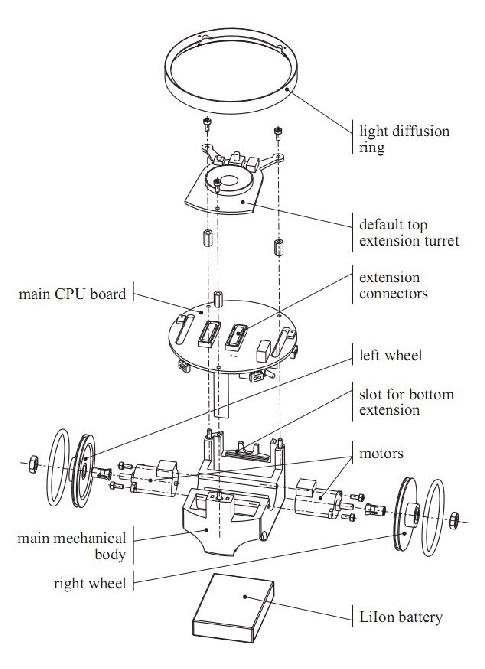
\includegraphics{epuck_str.pdf}}
    \end{picture}%
  \else
    \setlength{\unitlength}{1bp}%
    \begin{picture}(232.44, 320.96)(0,0)
    \put(0,0){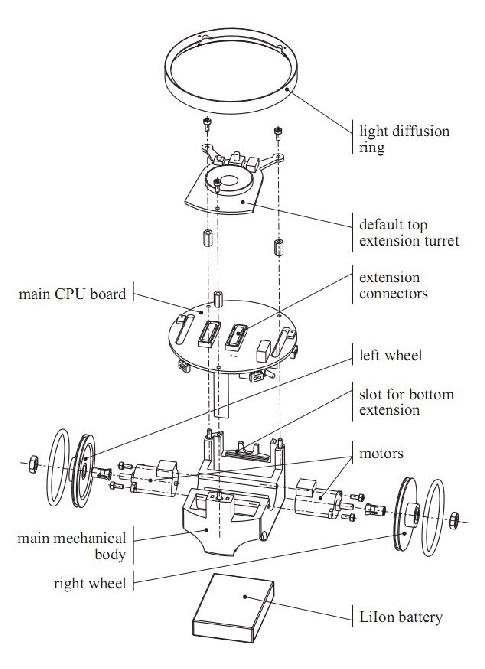
\includegraphics{epuck_str}}
    \end{picture}%
  \fi
  \caption{\label{pic:epuck_str}%
   Epuck structure \cite{robotica2009}}
  \end{figure}

  The mechanical design of e-Puck is shown in Figure ~\ref{pic:epuck_str}.
  It consists of a rounded transparent body, a battery, two stepper motors with
  wheels on their axis, a printed circuit board, plastic ring of LEDs, 
  a camera and a default extension board.
  There are extensions like floor sensors, a rotating scanner or a turret with linear cameras,
  which can scale up e-Puck's sensors. If we are talking about e-Puck in this thesis,
  it is meant e-Puck with the default extension only.
  
  A default robot is more than 60 mm 
  high and it has a diameter of 75 mm. 
  The battery is placed in the bottom and can be easily extracted and recharged separately.
  Two stepper motors with wheels are screwed to a plastic body and are located on axis of e-Puck
  in order to allow robot turn around on place. Wheels have the diameter of 41 mm and the perch is 53 mm.
  Printed circuit board is fixed to the top of the body and a ring of LEDs' is mounted around the board.
  A camera is placed on the front side of robot lying on the axis between the wheels.
  The extension board covers the main printed circuit board.
\section{Sensors, actuators and heart of the robot}
\label{sec:sencors}
  Sensors and actuators determine the possible robot usage.
  Luckily, e-Puck has a lot of sensors of different kinds and is equipped with typical actuators.
  The following paragraphs shortly describe e-Puck's sensors and actuators and mention a few problems 
  with transmitting data between the robot and PC using {\it BTCom}. {\it BTCom} protocol is used by {\it Elib},
  so {\it Elib} is to some extent dependent on {\it BTCom}.
  The actuators consist of motors, 8 red LEDs on perimeter, 4 green body LEDs,
   which are turned on/off together, a front LED and a speaker.
   
  Stepper motors are a great advantage of e-Puck, because the motion of wheel can be split
  into small steps. One wheel revolution corresponds to 1000 steps of motor. The 
  diameter of the wheel is 41 mm. If the wheel makes one revolution, the wheel goes 128.8 mm. 
  In conclusion a thousand of steps matches 128.8 mm of linear movement and one step is 0.1288 mm. 
  Motors are equipped with encoders and the motors are very accurate, 
  which in combination with simple odometry really helps in localization tasks.
  A nice feature of encoders is that their value can be set at any time.
  The maximum speed of the motors is one revolution per second in both directions.
  {\it BTCom} allows a programmer to set the speed of motors and also get and set the values
  of encoders.
   
  All e-Puck LEDs can be used for debugging or for making robot visible to other devices.
  Furthermore, the front LED is usually used to illuminate the terrain in front of  e-Puck.
  Each LED can be turned off, turned on or set to an inverse state.
  
  Three axis accelerometers are placed inside the robots body. In the rest position
  the accelerometers measure the slant of e-Puck. They can also measure acceleration of e-Puck
  and for example detect a collision or a falling state of e-Puck. 
%	There is no problem with using accelerometer via {\it BTCom}.
  
  Infra Red (IR) sensors are typical sensors for mobile robotics. E-Puck has eight of them.
  Four are located in the front part of e-Puck, two are on both sides, two on back side.
  Sensors work in two modes. First they measure ambient infra red light.
  In the second mode IR sensors emit IR light and they measure reflected light, so 
  they can detect close obstacles.
  Both functions are available in {\it BTCom}. 				
  Calibration of sensors increases the precision of detecting near obstacles.
  Infra red sensors are capable of recognising an obstacle at a distance 4 cm.
  
  The speaker together with microphones are suitable communication tools between
  the people and e-Puck.
  On the other hand, a limited processing power of e-Puck does not allow to store and
   play complicated sounds. It is also impossible to use a speaker with microphones to speech
   recognition due to insufficient processing power.
  Despite the limitation of processing power the microphones can be easily used to locate
  the source of sound via amplitude measurement, because the microphones are placed near the perimeter
  in a triangle. Microphones measure current amplitude of sound. As exact distances between microphones 
  are known, we can compute frequency of the sound using Fast Fourier Transformation (FFT).
  Digital Signal Processor (DSP) is suitable for computing FFT,
   which will be introduced below in this chapter.
  Maximal acquisition speed is 33 kHz. 
  For more information see \cite{sound}.
  
  A program which uses {\it BTCom} can capture values of amplitude only in irregular intervals, so 
  it is not possible to compute frequency of sound by running FFT on Personal Computer. 
  However to locate the source of sound is still possible.
  
  %\input{epuck.TpX}
  \begin{figure}[!hbp]
  \centering
  \ifpdf
    \setlength{\unitlength}{1bp}%
    \begin{picture}(228.66, 174.33)(0,0)
    \put(0,0){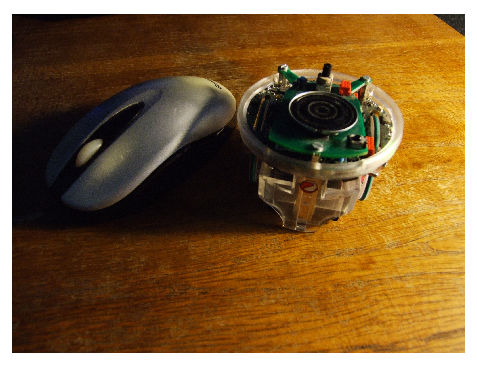
\includegraphics{epuck.pdf}}
    \end{picture}%
  \else
    \setlength{\unitlength}{1bp}%
    \begin{picture}(228.66, 174.33)(0,0)
    \put(0,0){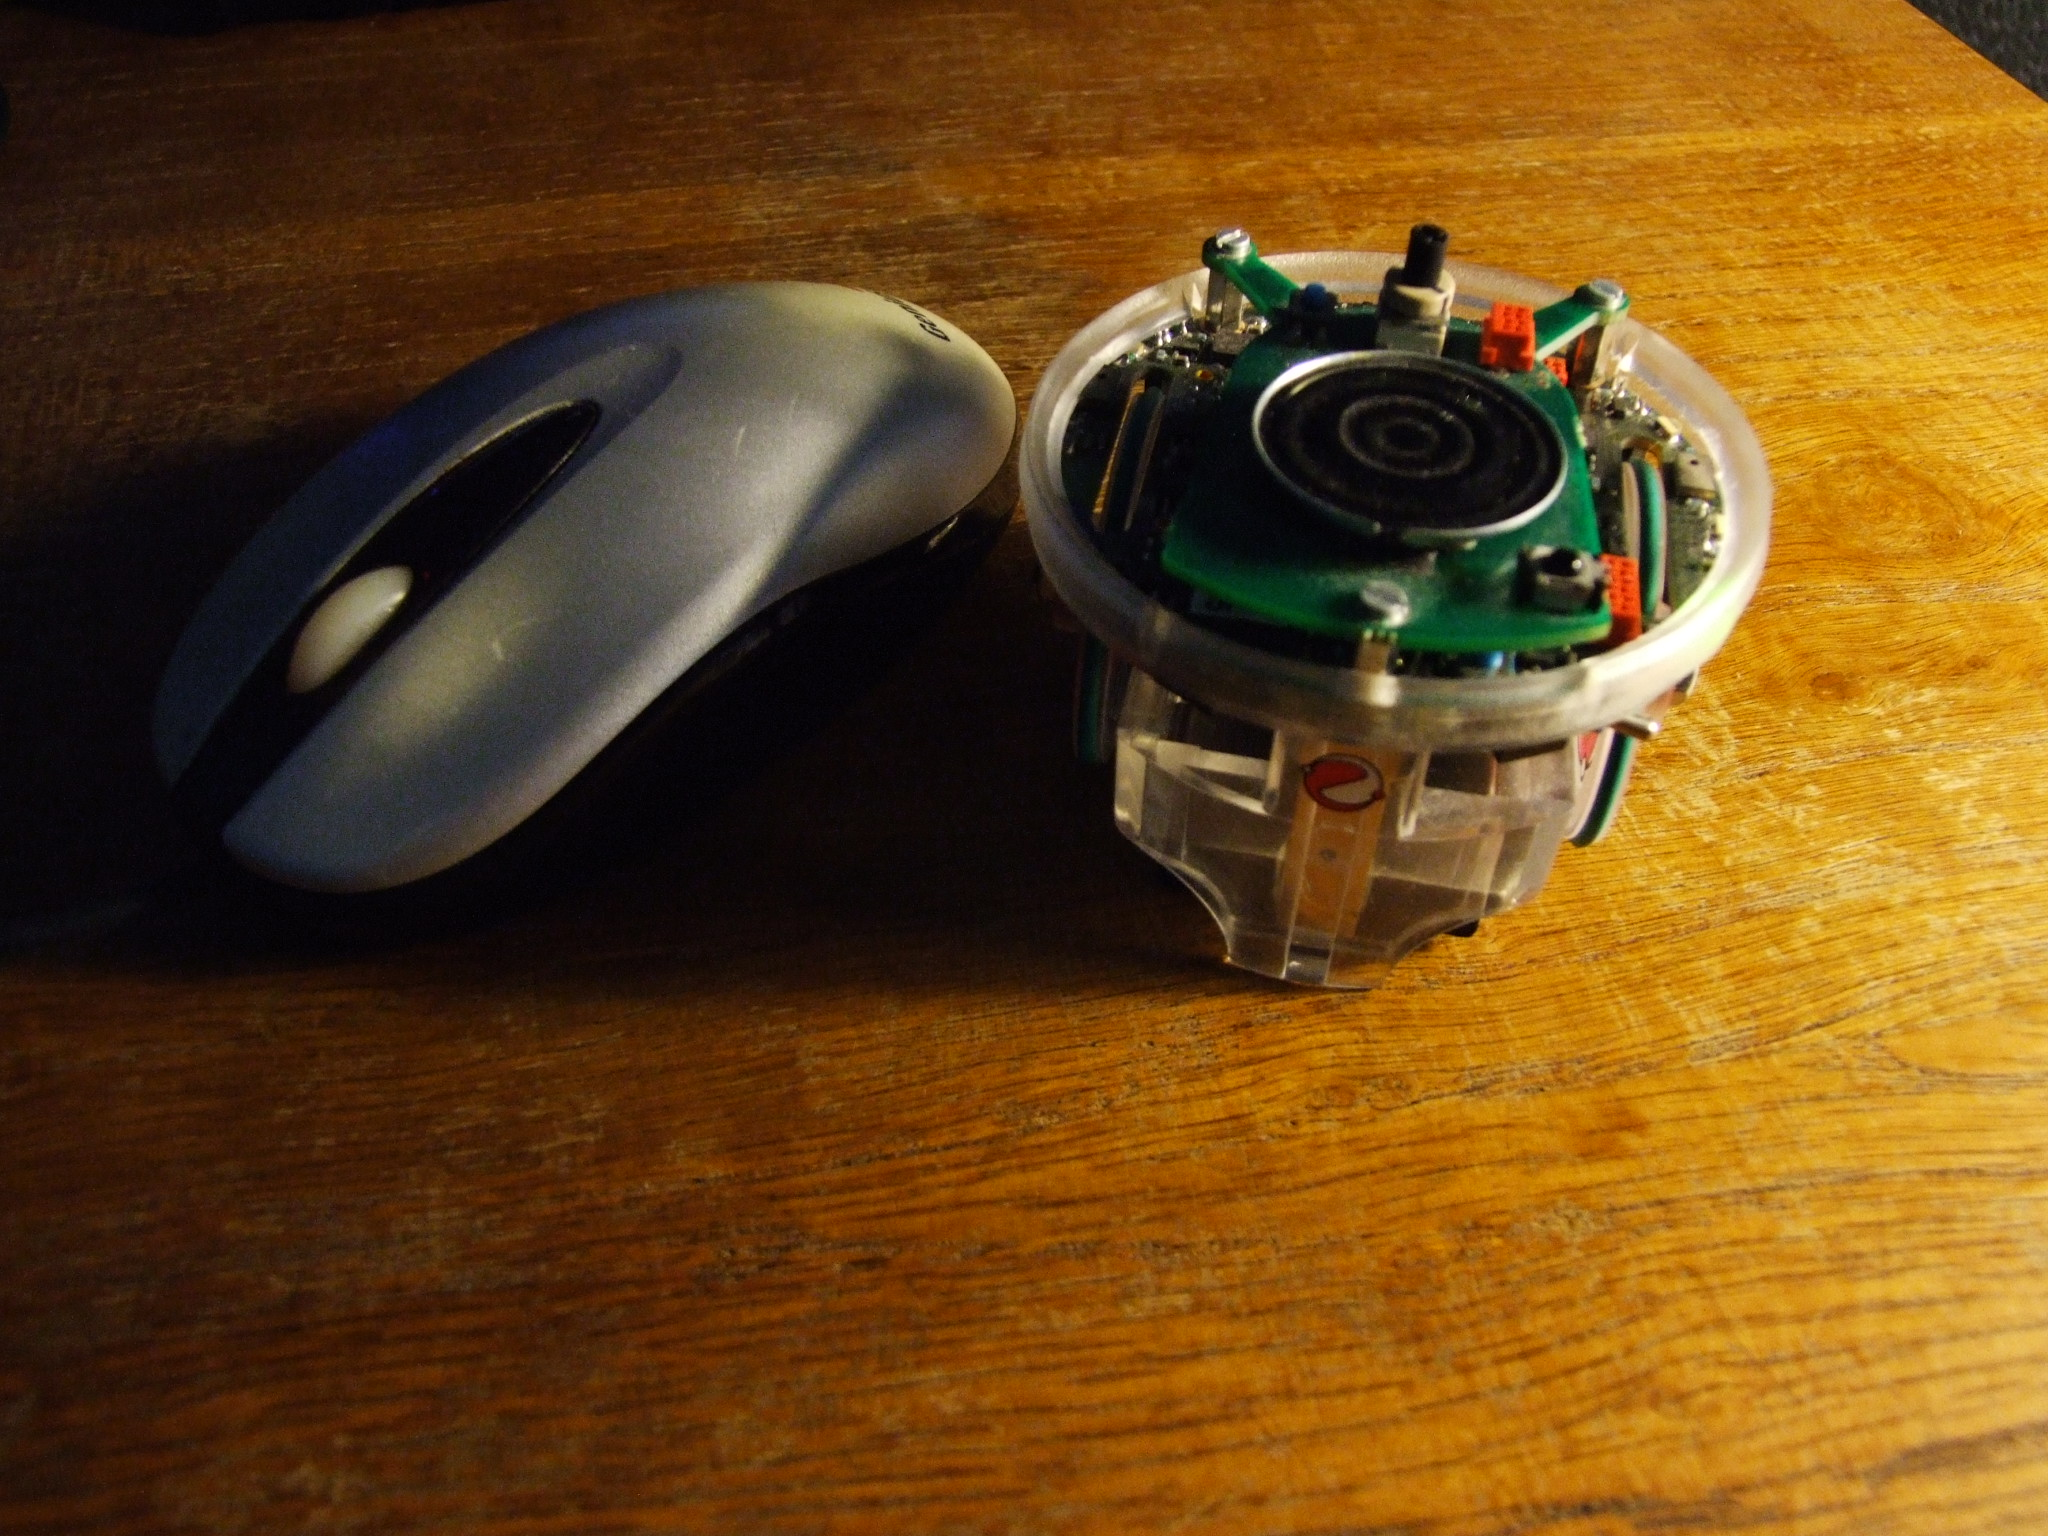
\includegraphics{epuck}}
    \end{picture}%
  \fi
  \caption{\label{pic:epuck}%
   E-Puck avoiding a mouse}
  \end{figure}

  E-Puck's camera is a colour CMOS camera with 640 * 480 resolution. 
  Because only 8 kB of RAM memory is available,
  the picture size has to be reduced in order to save the image in the memory.
  The image processing is really demanding on the processing power so it is not 
  convenient to be run on the slow e-Puck's processor.
  
  On the other hand, using {\it BTCom} solves the problem with limited processing power
  by sending picture to Personal Computer (PC). PC has enough resources to process the image fast,
   but the transport of an image takes a long time too. 
   For example capturing and sending a colour image of size 40 * 40 pixels 
  takes more than 0.2 seconds, if it is sent over Bluetooth.
  {\it BTCom} can set height, width, colour mode and zoom. A colour picture is twice as big as the same picture taken
  in grey scale mode.
  In the gray scale mode, each pixel is represented by 1 byte value of
  intensity. Each pixel of color picture is represented as 3 values of $RGB$
  stored in 2 bytes. Red color is stored in first 5 bits, green is represented
  by the next 6 bits, finally the last 5 bits of 2 bytes represents blue color.
  %can be seen in btcom.c protocol
   Zoom has three acceptable values 1, 4 and 8. One is for the biggest zoom, 8 represents the smallest.
  Width and height are limited only by the size of the available memory in e-Puck.
  
  Processor, dsPIC 30F6014, is the heart of e-Puck and runs at 60 MHz, which correspond to 15 MIPS.
  It has C oriented instructions and supports compiling from GNU compilers.
  Apart from standard 16 bits core unit Digital Signal Processor brings very high performance for computation,
  for example FFT or other signal processing.
  Programs can be downloaded to flash memory with 144 kB and
   are loaded to RAM memory according to the selector position.
  E-Puck's RAM memory has only 8 kB. A currently running program and all its data are placed in RAM memory.
  %todo IR port 
  Communication with other devices is provided by IR port or Bluetooth and RS232 serial interface.
  Both, Bluetooth and RS232, can be used to download programs to e-Puck's flash memory.
  In addition, Bluetooth can be used to communicate with other e-Pucks or with a computer
  using {\it BTCom}. 
  The counter part of {\it BTCom} on computer is connected to the serial port.


  \begin{figure}[!hbp]
  \centering
  \ifpdf
    \setlength{\unitlength}{1bp}%
    \begin{picture}(228.66, 174.33)(0,0)
    \put(0,0){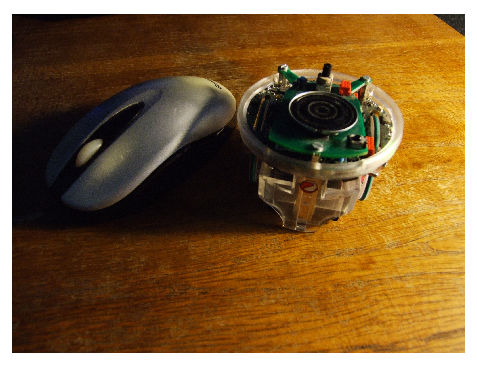
\includegraphics{epuck.pdf}}
    \end{picture}%
  \else
    \setlength{\unitlength}{1bp}%
    \begin{picture}(228.66, 174.33)(0,0)
    \put(0,0){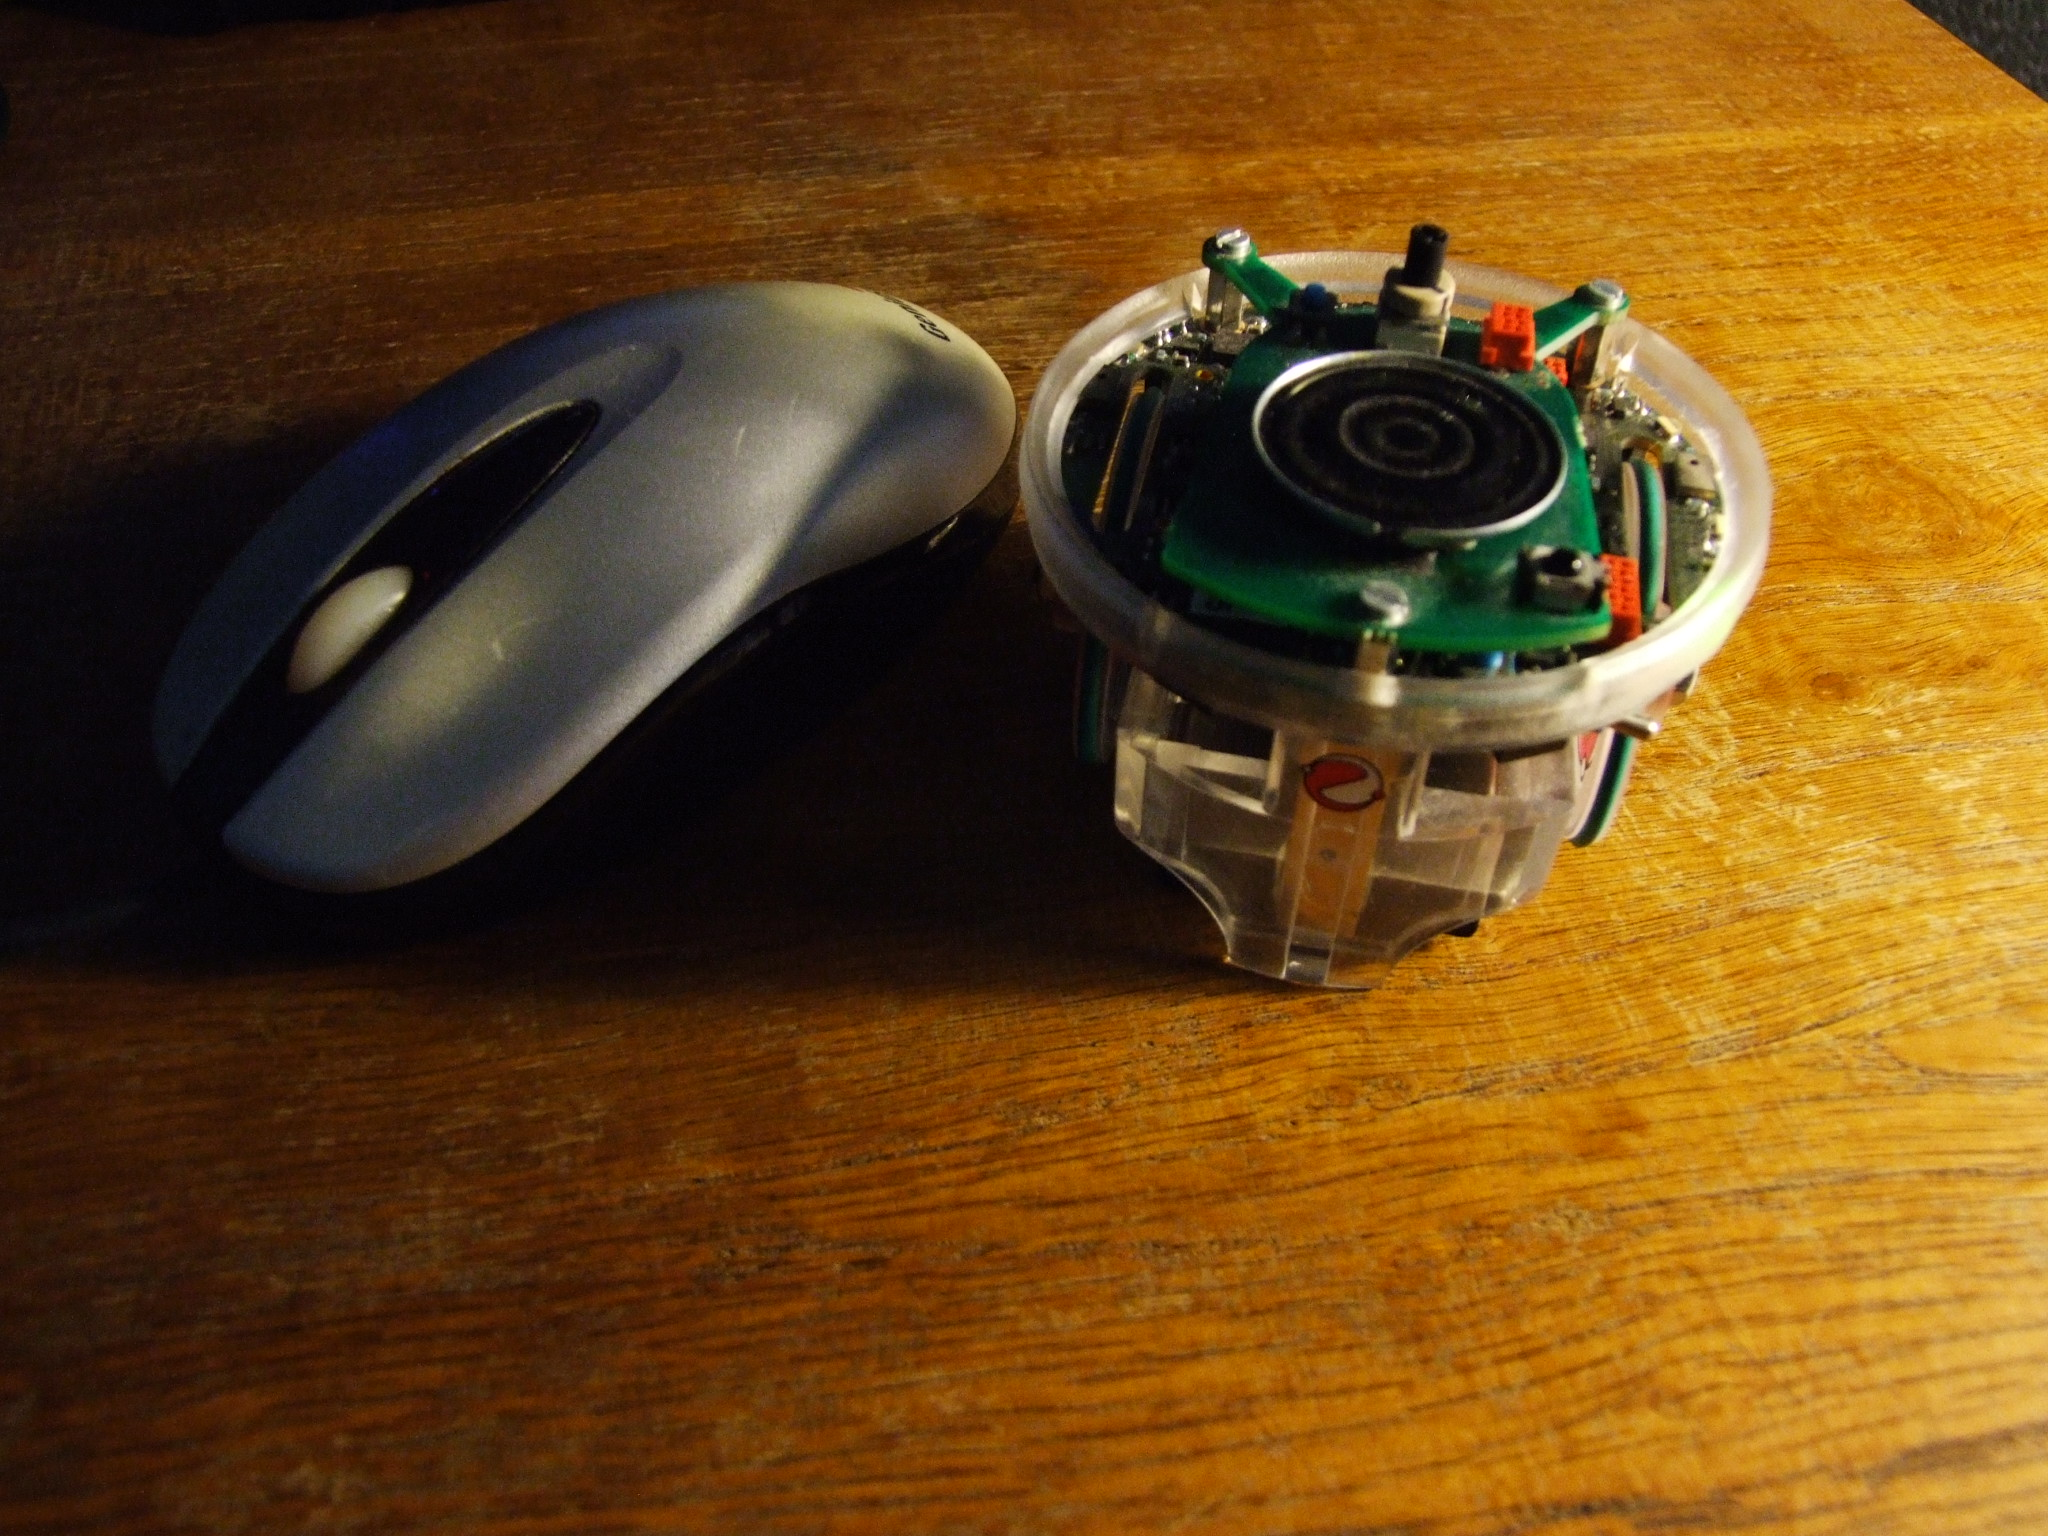
\includegraphics{epuck}}
    \end{picture}%
  \fi
  \caption{\label{pic:epuck}%
   E-Puck avoiding a mouse}
  \end{figure}

  E-Puck's camera is a colour CMOS camera with 640 * 480 resolution. 
  Because only 8 kB of RAM memory is available,
  the picture size has to be reduced in order to save the image in the memory.
  The image processing is really demanding on the processing power so it is not 
  convenient to be run on the slow e-Puck's processor.
  
  On the other hand, using {\it BTCom} solves the problem with limited processing power
  by sending picture to Personal Computer (PC). PC has enough resources to process the image fast,
   but the transport of an image takes a long time too. 
   For example capturing and sending a colour image of size 40 * 40 pixels 
  takes more than 0.2 seconds, if it is sent over Bluetooth.
  {\it BTCom} can set height, width, colour mode and zoom. A colour picture is twice as big as the same picture taken
  in grey scale mode.
  In the gray scale mode, each pixel is represented by 1 byte value of
  intensity. Each pixel of color picture is represented as 3 values of $RGB$
  stored in 2 bytes. Red color is stored in first 5 bits, green is represented
  by the next 6 bits, finally the last 5 bits of 2 bytes represents blue color.
  %can be seen in btcom.c protocol
   Zoom has three acceptable values 1, 4 and 8. One is for the biggest zoom, 8 represents the smallest.
  Width and height are limited only by the size of the available memory in e-Puck.
  
  Processor, dsPIC 30F6014, is the heart of e-Puck and runs at 60 MHz, which correspond to 15 MIPS.
  It has C oriented instructions and supports compiling from GNU compilers.
  Apart from standard 16 bits core unit Digital Signal Processor brings very high performance for computation,
  for example FFT or other signal processing.
  Programs can be downloaded to flash memory with 144 kB and
   are loaded to RAM memory according to the selector position.
  E-Puck's RAM memory has only 8 kB. A currently running program and all its data are placed in RAM memory.
  %todo IR port 
  Communication with other devices is provided by IR port or Bluetooth and RS232 serial interface.
  Both, Bluetooth and RS232, can be used to download programs to e-Puck's flash memory.
  In addition, Bluetooth can be used to communicate with other e-Pucks or with a computer
  using {\it BTCom}. 
  The counter part of {\it BTCom} on computer is connected to the serial port.


  \begin{figure}[!hbp]
  \centering
  \ifpdf
    \setlength{\unitlength}{1bp}%
    \begin{picture}(228.66, 174.33)(0,0)
    \put(0,0){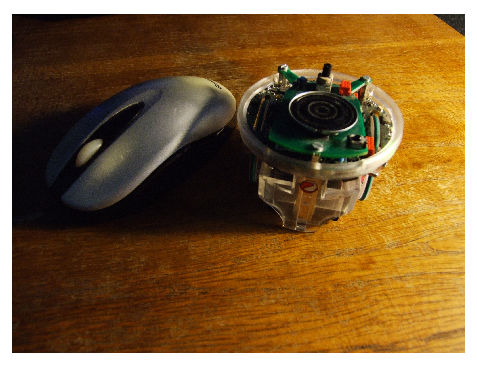
\includegraphics{epuck.pdf}}
    \end{picture}%
  \else
    \setlength{\unitlength}{1bp}%
    \begin{picture}(228.66, 174.33)(0,0)
    \put(0,0){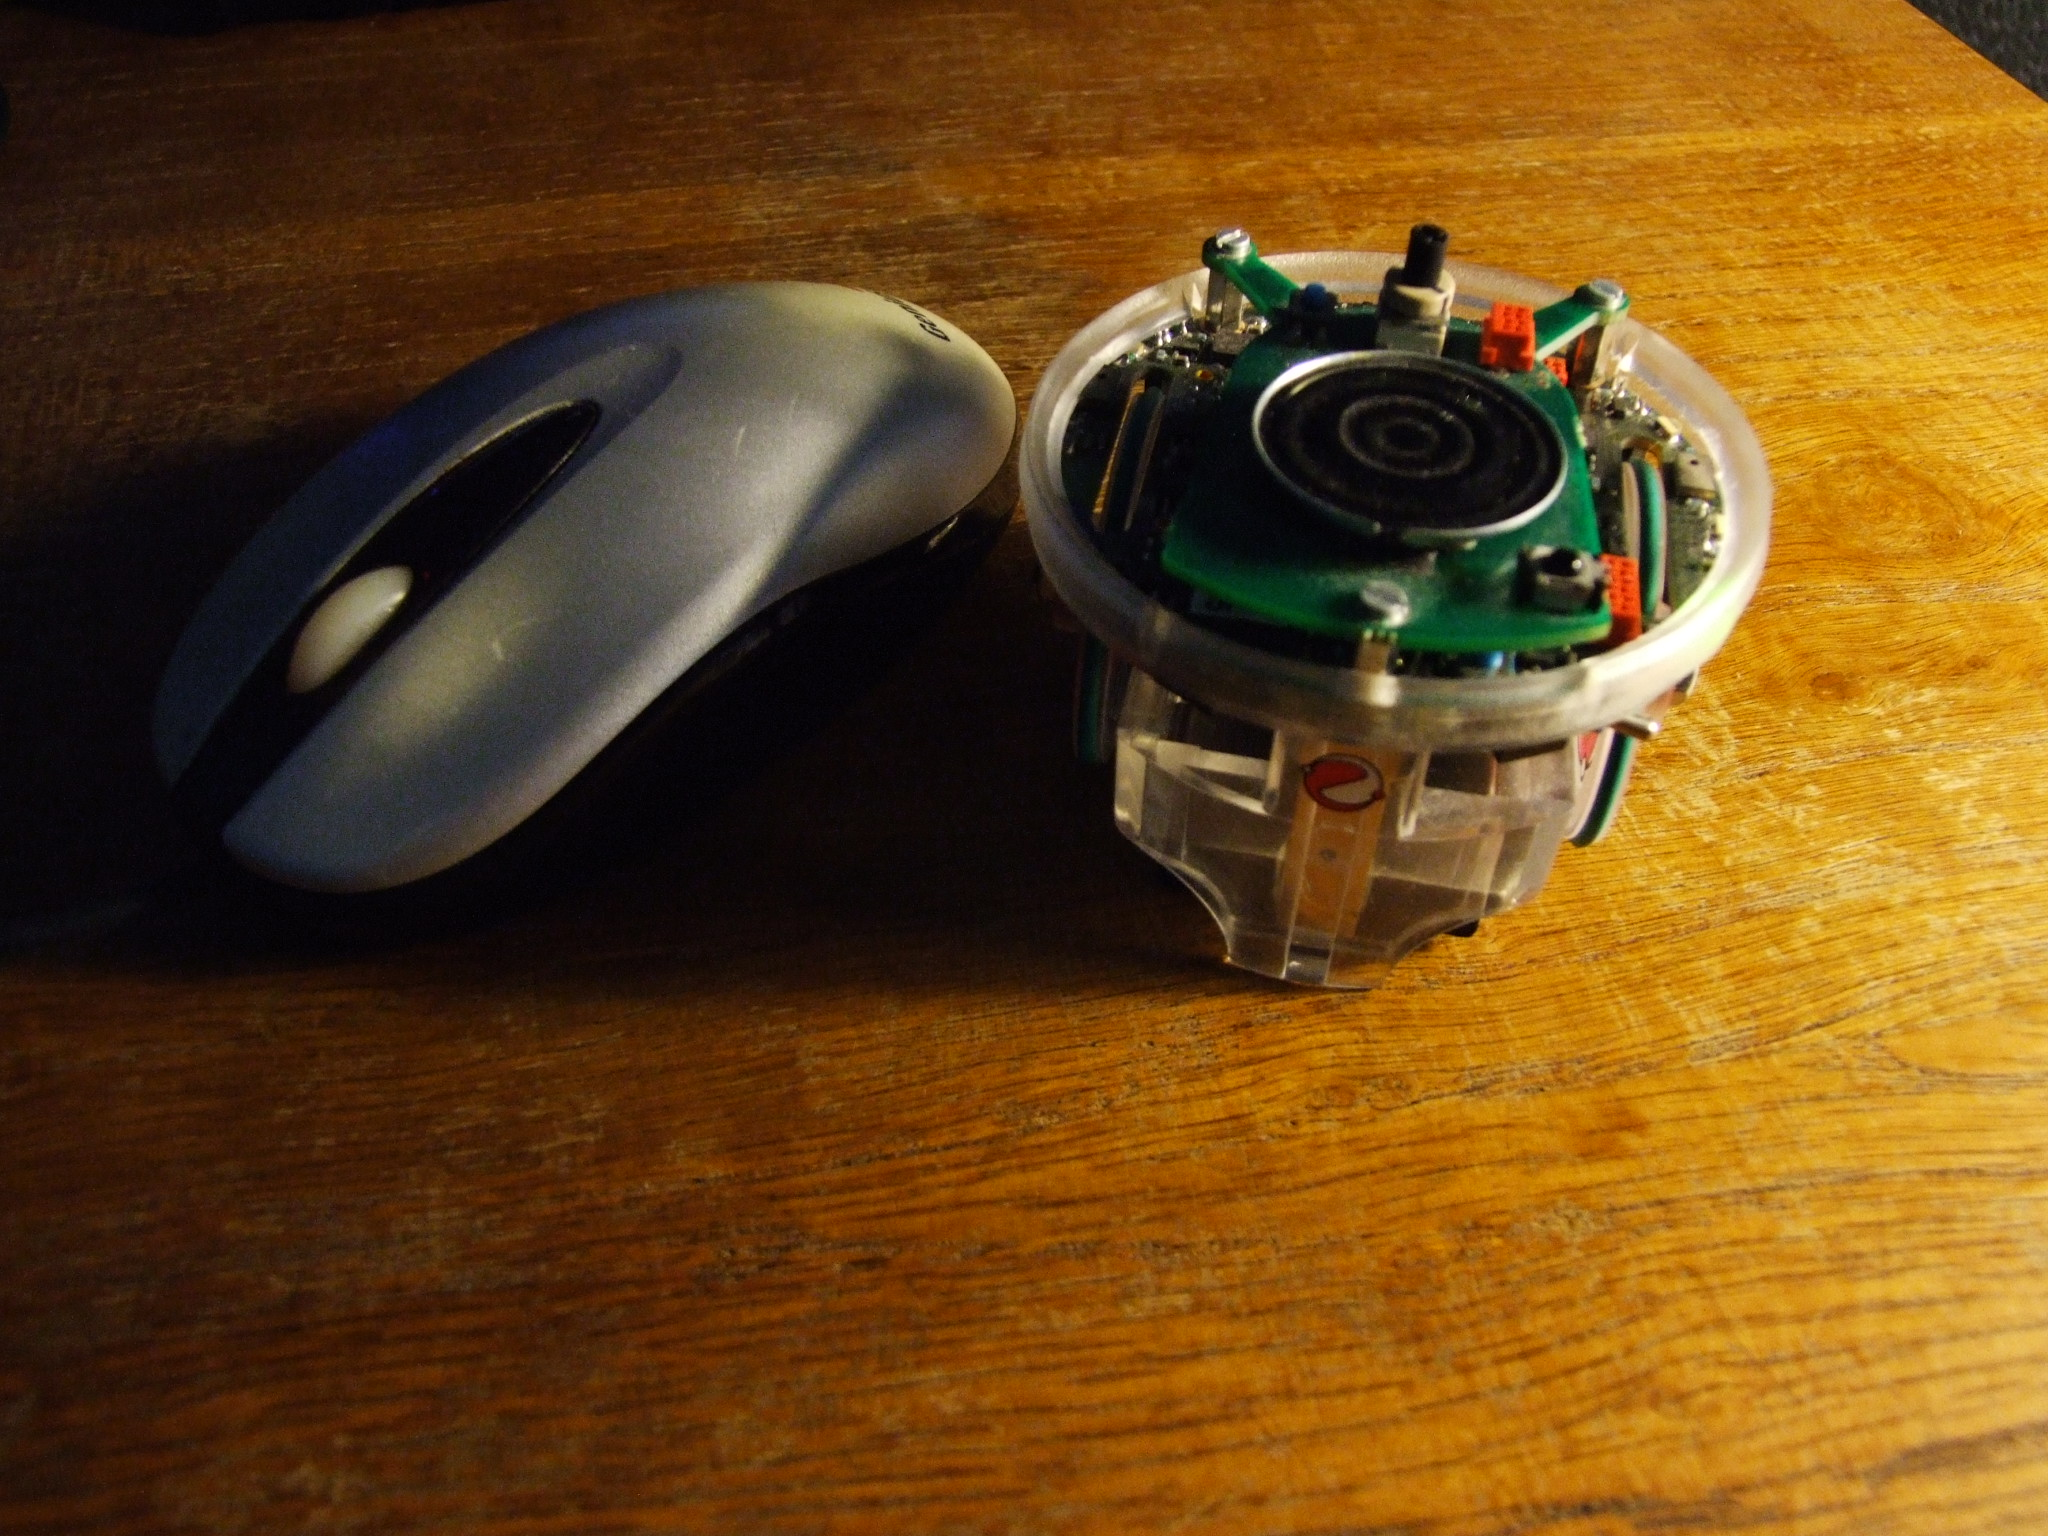
\includegraphics{epuck}}
    \end{picture}%
  \fi
  \caption{\label{pic:epuck}%
   E-Puck avoiding a mouse}
  \end{figure}

  E-Puck's camera is a colour CMOS camera with 640 * 480 resolution. 
  Because only 8 kB of RAM memory is available,
  the picture size has to be reduced in order to save the image in the memory.
  The image processing is really demanding on the processing power so it is not 
  convenient to be run on the slow e-Puck's processor.
  
  On the other hand, using {\it BTCom} solves the problem with limited processing power
  by sending picture to Personal Computer (PC). PC has enough resources to process the image fast,
   but the transport of an image takes a long time too. 
   For example capturing and sending a colour image of size 40 * 40 pixels 
  takes more than 0.2 seconds, if it is sent over Bluetooth.
  {\it BTCom} can set height, width, colour mode and zoom. A colour picture is twice as big as the same picture taken
  in grey scale mode.
  In the gray scale mode, each pixel is represented by 1 byte value of
  intensity. Each pixel of color picture is represented as 3 values of $RGB$
  stored in 2 bytes. Red color is stored in first 5 bits, green is represented
  by the next 6 bits, finally the last 5 bits of 2 bytes represents blue color.
  %can be seen in btcom.c protocol
   Zoom has three acceptable values 1, 4 and 8. One is for the biggest zoom, 8 represents the smallest.
  Width and height are limited only by the size of the available memory in e-Puck.
  
  Processor, dsPIC 30F6014, is the heart of e-Puck and runs at 60 MHz, which correspond to 15 MIPS.
  It has C oriented instructions and supports compiling from GNU compilers.
  Apart from standard 16 bits core unit Digital Signal Processor brings very high performance for computation,
  for example FFT or other signal processing.
  Programs can be downloaded to flash memory with 144 kB and
   are loaded to RAM memory according to the selector position.
  E-Puck's RAM memory has only 8 kB. A currently running program and all its data are placed in RAM memory.
  %todo IR port 
  Communication with other devices is provided by IR port or Bluetooth and RS232 serial interface.
  Both, Bluetooth and RS232, can be used to download programs to e-Puck's flash memory.
  In addition, Bluetooth can be used to communicate with other e-Pucks or with a computer
  using {\it BTCom}. 
  The counter part of {\it BTCom} on computer is connected to the serial port.


  \begin{figure}[!hbp]
  \centering
  \ifpdf
    \setlength{\unitlength}{1bp}%
    \begin{picture}(228.66, 174.33)(0,0)
    \put(0,0){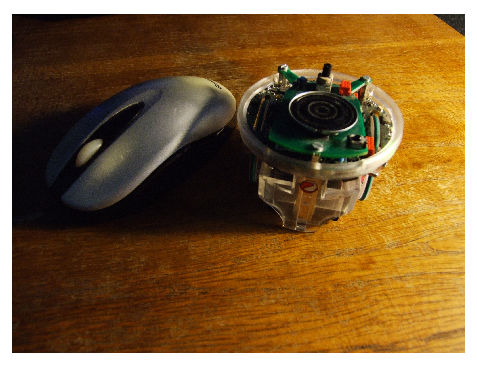
\includegraphics{epuck.pdf}}
    \end{picture}%
  \else
    \setlength{\unitlength}{1bp}%
    \begin{picture}(228.66, 174.33)(0,0)
    \put(0,0){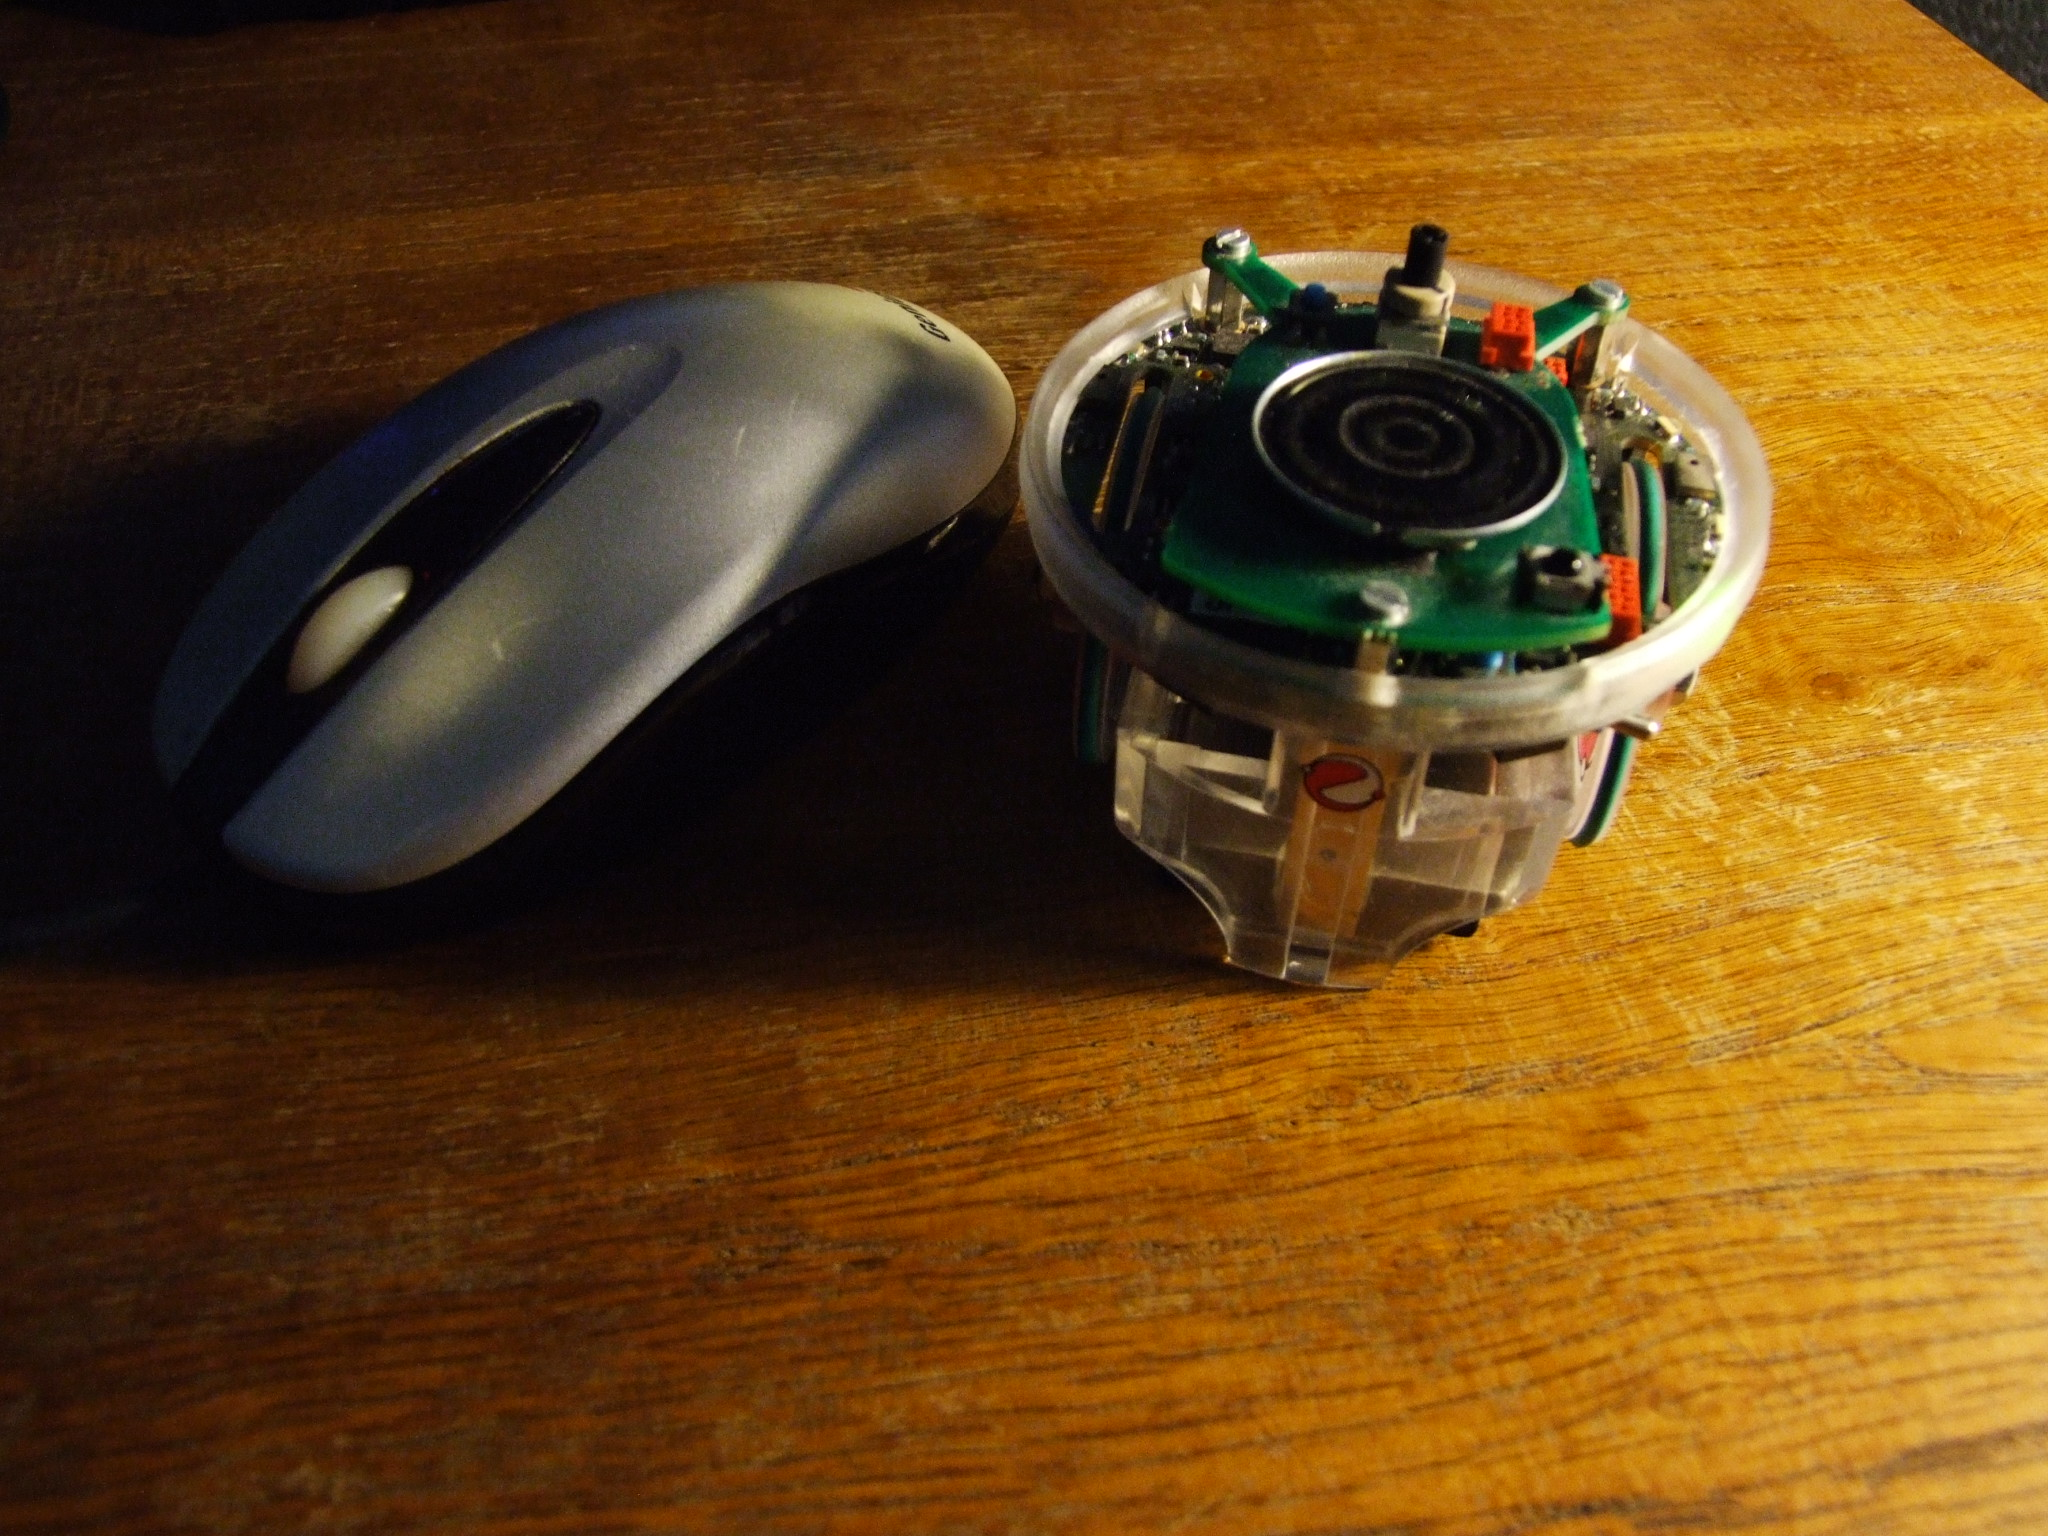
\includegraphics{epuck}}
    \end{picture}%
  \fi
  \caption{\label{pic:epuck}%
   E-Puck avoiding a mouse}
  \end{figure}

  E-Puck's camera is a colour CMOS camera with 640 * 480 resolution. 
  Only 8 kB of RAM memory is available, so the~size of an image has to be reduced in order to save the picture in the memory.
  The image processing is really demanding on the processing power so it is not 
  convenient to be run on the slow e-Puck's processor.
  
  On the other hand, using {\it BTCom} solves the problem with limited processing power
  by sending picture to Personal Computer (PC). PC has enough resources to process the image fast,
   but the transport of an image takes a long time too. 
   For example capturing and sending a colour image of size 40 * 40 pixels 
  takes around 0.3 seconds, if it is sent over Bluetooth.

  {\it BTCom} can set height, width, colour mode and zoom of camera. 
  A colour picture is twice as big as the same picture taken
  in grey scale mode.
  In the gray scale mode, each pixel is represented by 1 byte value of
  intensity. Each pixel of color picture is represented as 3 values of $RGB$
  stored in 2 bytes. Red color is stored in first 5 bits, green is represented
  by the next 6 bits, finally the last 5 bits of 2 bytes represents blue color.
  %can be seen in btcom.c protocol
   Zoom has three acceptable values 1, 4 and 8. One is for the biggest zoom, 8 represents the smallest.
  Width and height are limited only by the size of the available memory in e-Puck.
  
  Processor, dsPIC 30F6014, is the heart of e-Puck and runs at 60 MHz, which correspond to 15 MIPS.
  It has C oriented instructions and supports compiling from GNU compilers.
  Apart from standard 16 bits core unit, Digital Signal Processor brings very high performance for computation
  FFT or other signal processing.
  Programs can be downloaded to flash memory with 144 kB and
   are loaded to RAM memory according to the selector position.
  E-Puck's RAM memory has only 8 kB. A currently running program and all its data are placed in RAM memory.
  %todo IR port 
  Communication with other devices is provided by IR port or Bluetooth and RS232 serial interface.
  Both, Bluetooth and RS232, can be used to download programs to e-Puck's flash memory.
  In addition, Bluetooth can be used to communicate with other e-Pucks or with a computer
  using {\it BTCom}. 
  The counter part of {\it BTCom} on computer is connected to the serial port.

